% Created 2014-02-07 Fri 18:12
\documentclass[sans,aspectratio=169,presentation,bigger,fleqn]{beamer}
\usepackage[utf8]{inputenc}
\usepackage[T1]{fontenc}
\usepackage{fixltx2e}
\usepackage{graphicx}
\usepackage{longtable}
\usepackage{float}
\usepackage{wrapfig}
\usepackage{rotating}
\usepackage[normalem]{ulem}
\usepackage{amsmath}
\usepackage{textcomp}
\usepackage{marvosym}
\usepackage{wasysym}
\usepackage{amssymb}
\usepackage{hyperref}
\tolerance=1000
\usepackage{setspace}
\setstretch{1.3}
\usepackage{booktabs}
\hypersetup{colorlinks=true,linkcolor=blue,urlcolor=blue}
%\usetheme{naked}
\usepackage{lmodern}
\usetheme[alternativetitlepage=true,titleline=true]{Torino}
\usecolortheme{freewilly}
\usetheme{default}
\author{John Henderson}
\date{08 February 2014}
\title{An introduction to Shiny}
\hypersetup{
  pdfkeywords={},
  pdfsubject={},
  pdfcreator={Emacs 24.3.1 (Org mode 8.2.5h)}}
\begin{document}

\maketitle

\begin{frame}[fragile,label=sec-1]{Intro}
 \begin{itemize}
\item \texttt{shiny} is an \texttt{R} package that enables web based applications
\item Overview of \texttt{shiny} basics
\item Two examples
\item The code/data necessary to reproduce anything in this talk is all on \href{https://github.com/jwhendy/devFest-shiny}{github}
\end{itemize}
\end{frame}
\begin{frame}[fragile,label=sec-2]{Basics}
 \begin{itemize}
\item \texttt{shiny} works inside of \href{http://www.rstudio.com/}{RStudio}

\item Two files are required to run an application
\item \texttt{ui.R}: sets page format, user input elements, and outputs you're going to create
\item \texttt{server.R}: contains the R code which will generate your dynamic output
\end{itemize}

\vspace{0.5cm}

Don't forget to run \texttt{install.packages("shiny")}!
\end{frame}
\begin{frame}[fragile,label=sec-3]{Minimal \texttt{ui.R}}
 \scriptsize
\begin{verbatim}
library(shiny)
# page format
shinyUI(pageWithSidebar(
  # title
  headerPanel("Hello Shiny!"),

  sidebarPanel(
    # user inputs go here
  ),

  mainPanel(
    plotOutput("plot") # what you're going to output, e.g. a plot
  )
))
\end{verbatim}
\scriptsize
\end{frame}
\begin{frame}[fragile,label=sec-4]{Minimal \texttt{server.R}}
 \scriptsize
\begin{verbatim}
library(shiny)

shinyServer(function(input, output) {

  # general R code here: load libraries, set variables/functions/etc.

  # output$name has to match ui.R's plotOutput("name")
  output$plot <- renderPlot({

    # code to make a plot goes here

  })
})
\end{verbatim}
\scriptsize
\end{frame}
\begin{frame}[fragile,label=sec-5]{It works!}
 \begin{itemize}
\item After defining the above files\ldots{}
\end{itemize}

\scriptsize
\begin{verbatim}
# run from within R studio
library(shiny)
setwd("/path/to/ui-and-server.R")
runApp()
\end{verbatim}

\begin{center}
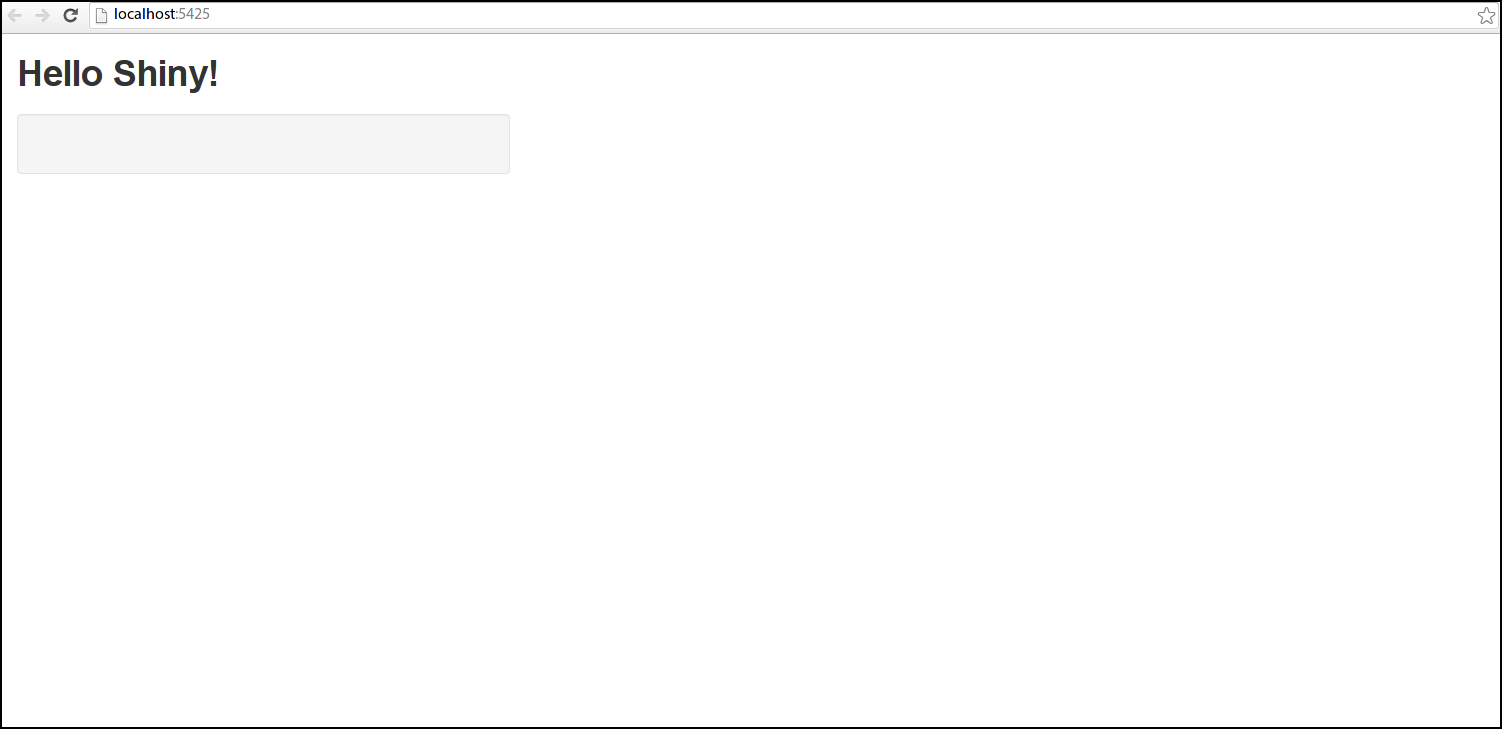
\includegraphics[height=3.75cm]{./img/shiny-template.png}
\end{center}
\end{frame}
\begin{frame}[label=sec-6]{Example: data analysis/exploration}
\begin{itemize}
\item Enable rapid and dynamic switching of plot variables
\item Allows for rapid plot prototyping to examine trends/relationships
\item Web-based solution is easily sharable with others
\end{itemize}
\end{frame}
\begin{frame}[fragile,label=sec-7]{Fiddling with public transportation data}
 \begin{itemize}
\item Grabbed/cleaned data on public transportation centers around US
\item Some are quite efficient, some are horrible
\item Can \texttt{shiny} help find some interesting tidbits?
\end{itemize}

\pause

\alert{Demo time!}
\end{frame}
\begin{frame}[label=sec-8]{Example: visualizing insurance costs}
\begin{itemize}
\item Benefit plan choices are hard; getting harder
\item Started making visualizations/walkthroughs in 2011
\item Goal: simplify decision making process at 3M
\end{itemize}
\end{frame}

\begin{frame}[label=sec-9]{In general, insurance is simple}
There are three "phases" of employee out of pocket expenses:
\begin{itemize}
\item If the \alert{deductible} has not been met, employee pays in full
\item Once deductible is met, employee pays 10\% coinsurance
\item When \alert{\(OOP_{max}\)} is reached, the employee pays nothing further
\end{itemize}

\vspace{0.5cm}

To find \(OOP_{max}\)

\footnotesize
\[
OOP_{max} = Ded + (0.1 \times (Exp_{max} - Ded)) \; ; \; \frac{OOP_{max} - Ded}{0.1} + Ded
\]
\normalsize
\end{frame}
\begin{frame}[label=sec-10]{2011: it was simple back then}
\begin{itemize}
\item What employees are given\ldots{} which plan is best?
\end{itemize}

\begin{center}
\begin{tabular}{lll}
\toprule
 & Plan A & Plan B\\
\midrule
Premium & \$150/mo & \$250/mo\\
3M Contribution & \$1,000 & \$0\\
Deductible & \$2,500 & \$750\\
\(OOP_{max}\) & \$5,000 & \$4,000\\
\bottomrule
\end{tabular}
\end{center}
\end{frame}
\begin{frame}[label=sec-11]{Perhaps math makes it easier?}
Let \(I(x)\) represent \(OOP\) over a range of \(Expenses\):

\footnotesize
\setlength{\mathindent}{0cm}
\[
I(x) = \begin{cases}
Expenses & \text{if} \quad 0 < x < Ded \\
Ded + (0.10 \times (Expenses - Ded)) & \text{if} \quad Ded  \le x <  Expenses_{max} \\     
OOP_{max} & \text{if} \quad Expenses_{max} \le x < \infty
\end{cases}
\]
\normalsize
\end{frame}
\begin{frame}[label=sec-12]{But doesn't visualization take the cake?}
\begin{itemize}
\item Cost, apparent
\end{itemize}

\begin{center}
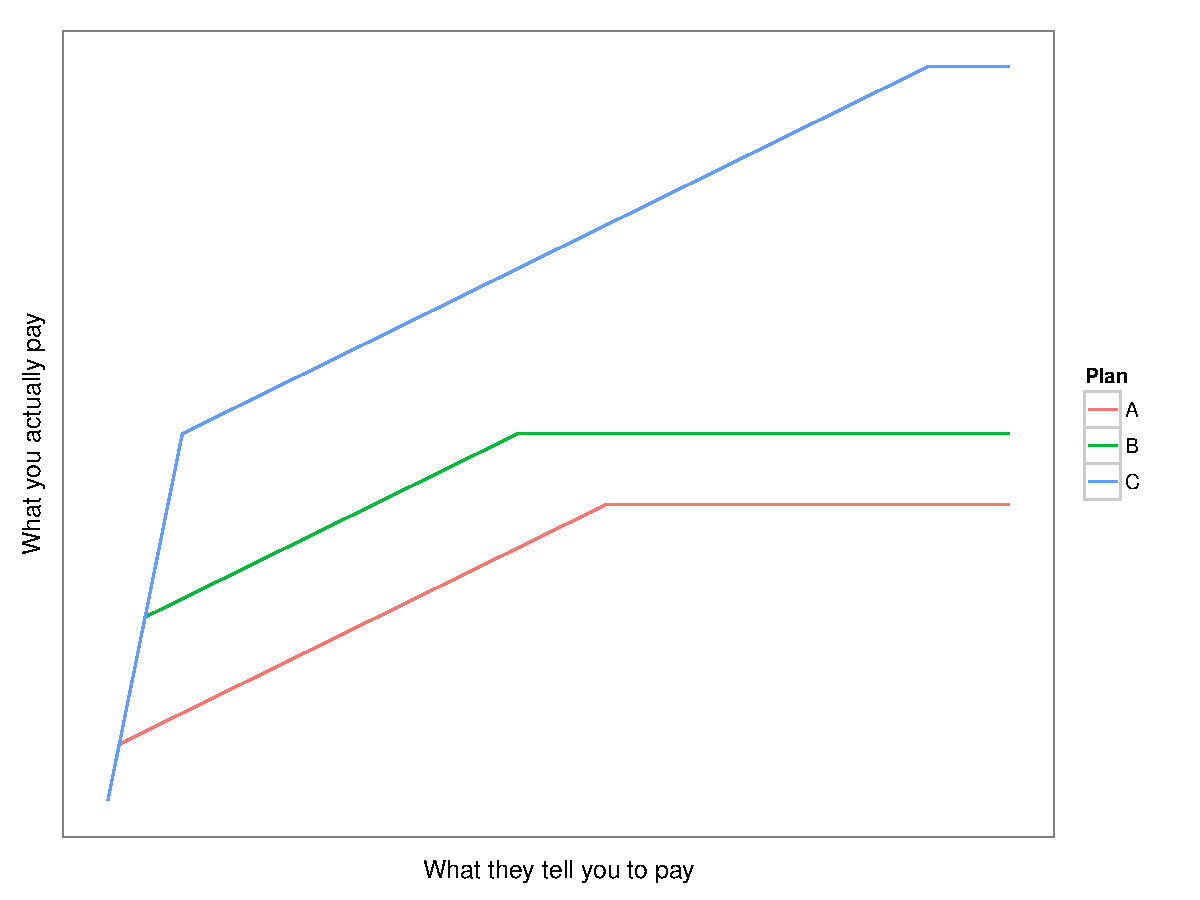
\includegraphics[height=6cm]{./img/ins-apparent.pdf}
\end{center}
\end{frame}
\begin{frame}[label=sec-13]{But doesn't visualization take the cake?}
\begin{itemize}
\item Cost, adjusted for company HSA contribution
\end{itemize}

\begin{center}
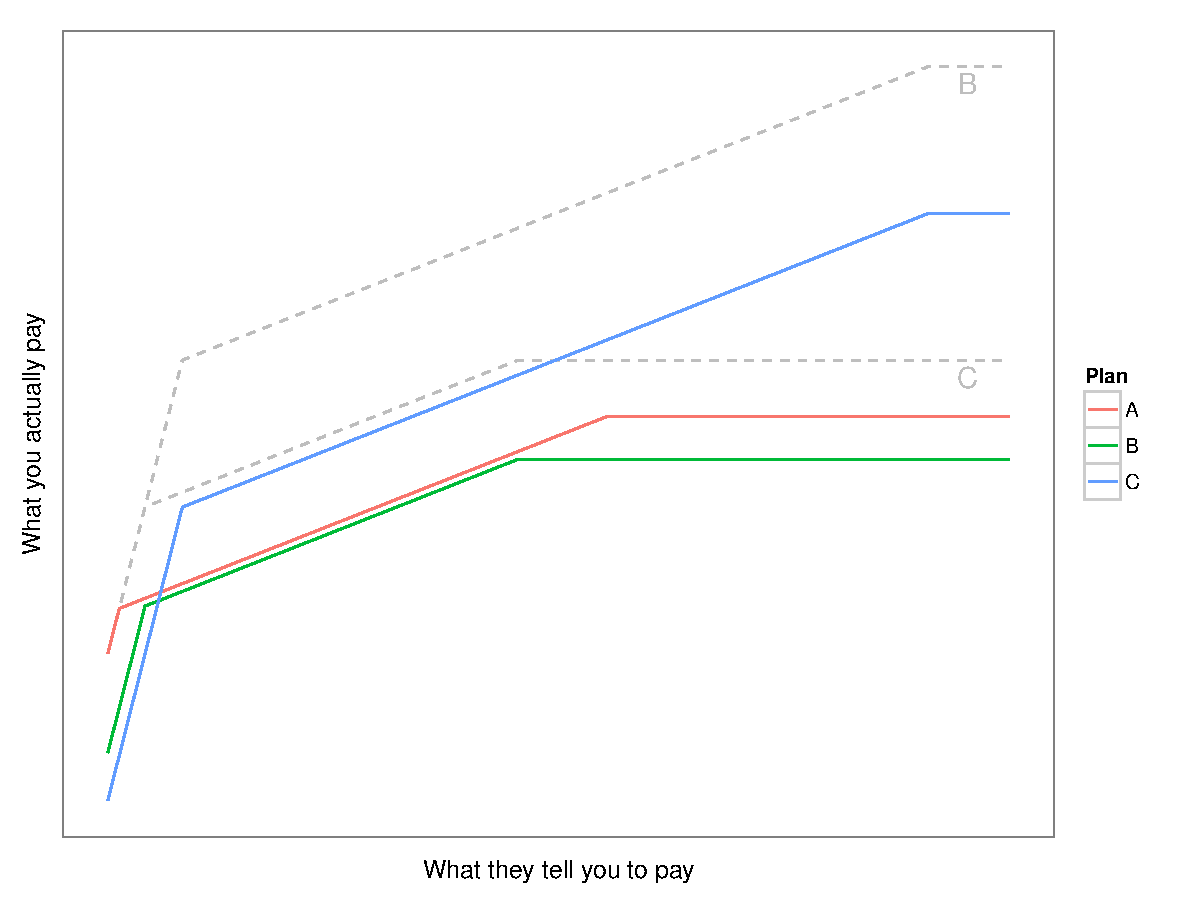
\includegraphics[height=6cm]{./img/ins-adjusted.pdf}
\end{center}
\end{frame}

\begin{frame}[label=sec-14]{But doesn't visualization take the cake?}
\begin{itemize}
\item Handy dandy intersection points
\end{itemize}

\begin{center}
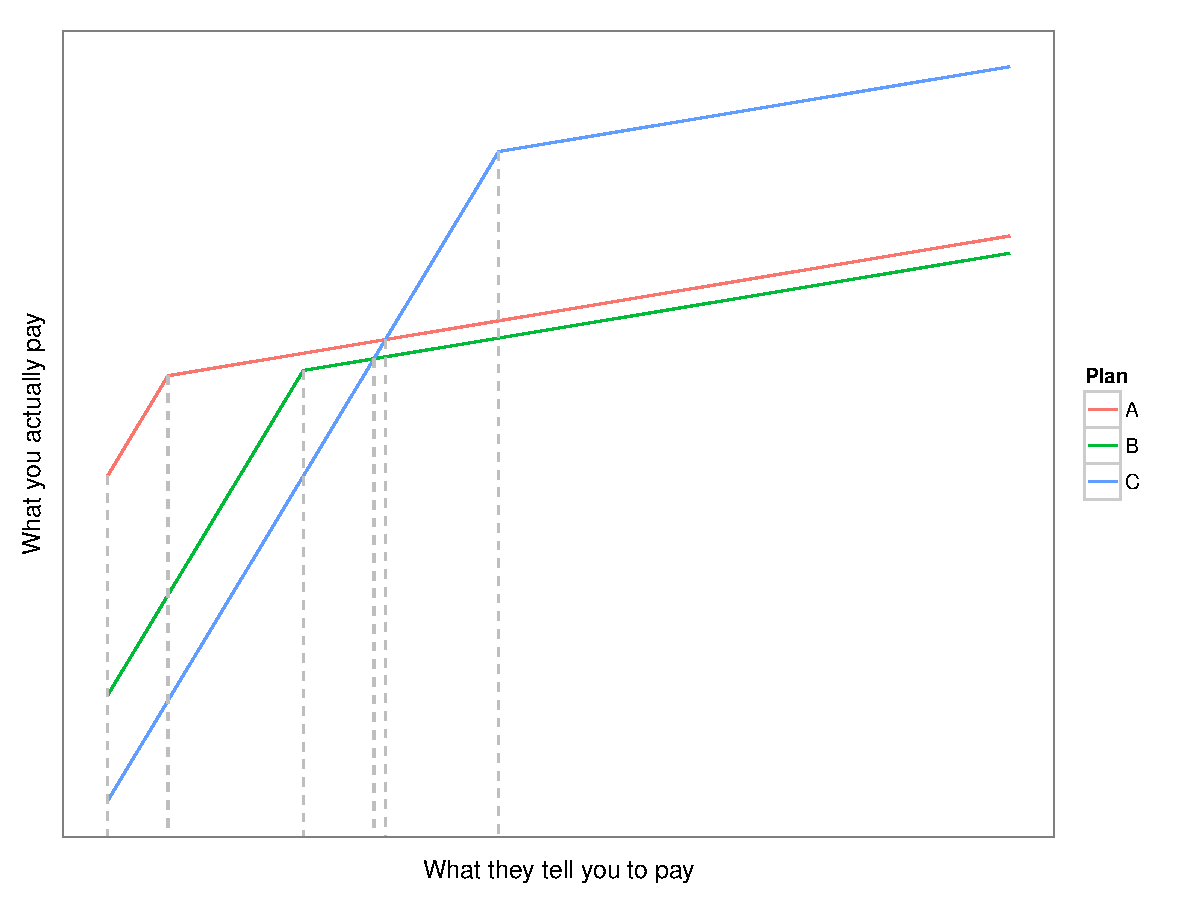
\includegraphics[height=6cm]{./img/ins-intersections.pdf}
\end{center}
\end{frame}

\begin{frame}[label=sec-15]{Let's go all n-dimensional}
Split deductible system for Plans B and C
\begin{itemize}
\item If a single individual reaches \(Ded_{ind}\), he/she covered at 90\%
\item Whole family covered when \(Ded_{fam}\) is met
\item Similarly, \(OOP_{max}\) is split (\(OOP_{max-ind}\) and \(OOP_{max-fam}\))
\end{itemize}

\vspace{0.25cm}

For example:
\begin{itemize}
\item Assume only one family member incurs any medical expenses
\item Individual covered at 90\% once \(Ded_{ind}\) is reached
\item Costs capped for individual once the \emph{individual} \(OOP_{max}\) is met
\end{itemize}
\end{frame}
\begin{frame}[label=sec-16]{Still so simple?}
\begin{itemize}
\item Now which plan is best?
\end{itemize}

\scriptsize
\begin{center}
\begin{tabular}{lllllll}
\toprule
Plan & Premium & \(Ded_{ind}\) & \(Ded_{tot}\) & \(OOP_{ind}\) & \(OOP_{tot}\) & \(HSA\)\\
\midrule
A & \$3,120 & \$400 & \$800 & \$2,100 & \$4,200 & -\\
B & \$2,088 & - & \$2,600 & - & \$5,200 & \$1,200\\
C & \$504 & \$2,600 & \$5,200 & \$5,200 & \$10,400 & \$1,200\\
\bottomrule
\end{tabular}
\end{center}
\normalsize
\end{frame}
\begin{frame}[label=sec-17]{First shot}
\begin{itemize}
\item Contour of highest spender vs. everyone else
\end{itemize}

\begin{center}
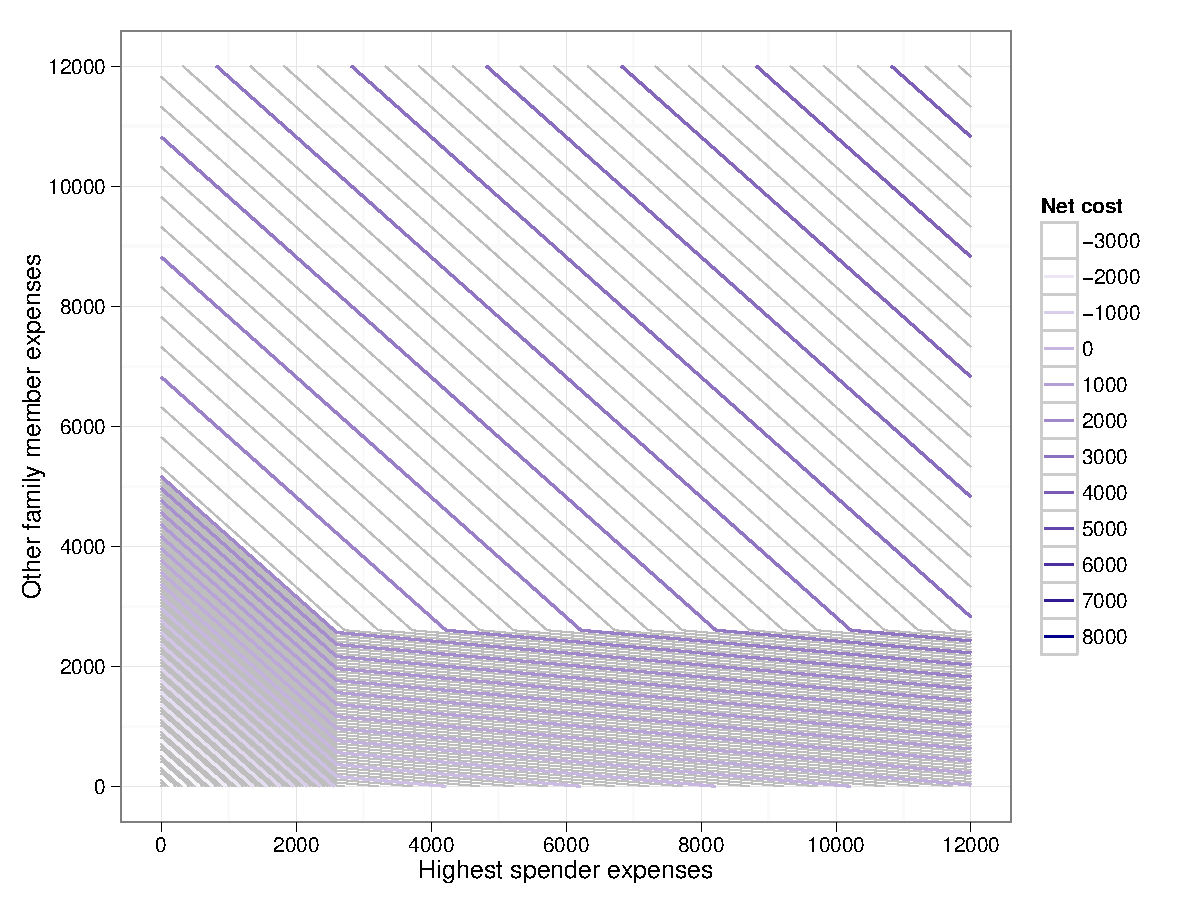
\includegraphics[height=6cm]{./img/ins-contour.pdf}
\end{center}
\end{frame}

\begin{frame}[label=sec-18]{Winning cost map}
\begin{itemize}
\item "Stack" the contours, figure out which one is lowest
\end{itemize}

\begin{center}
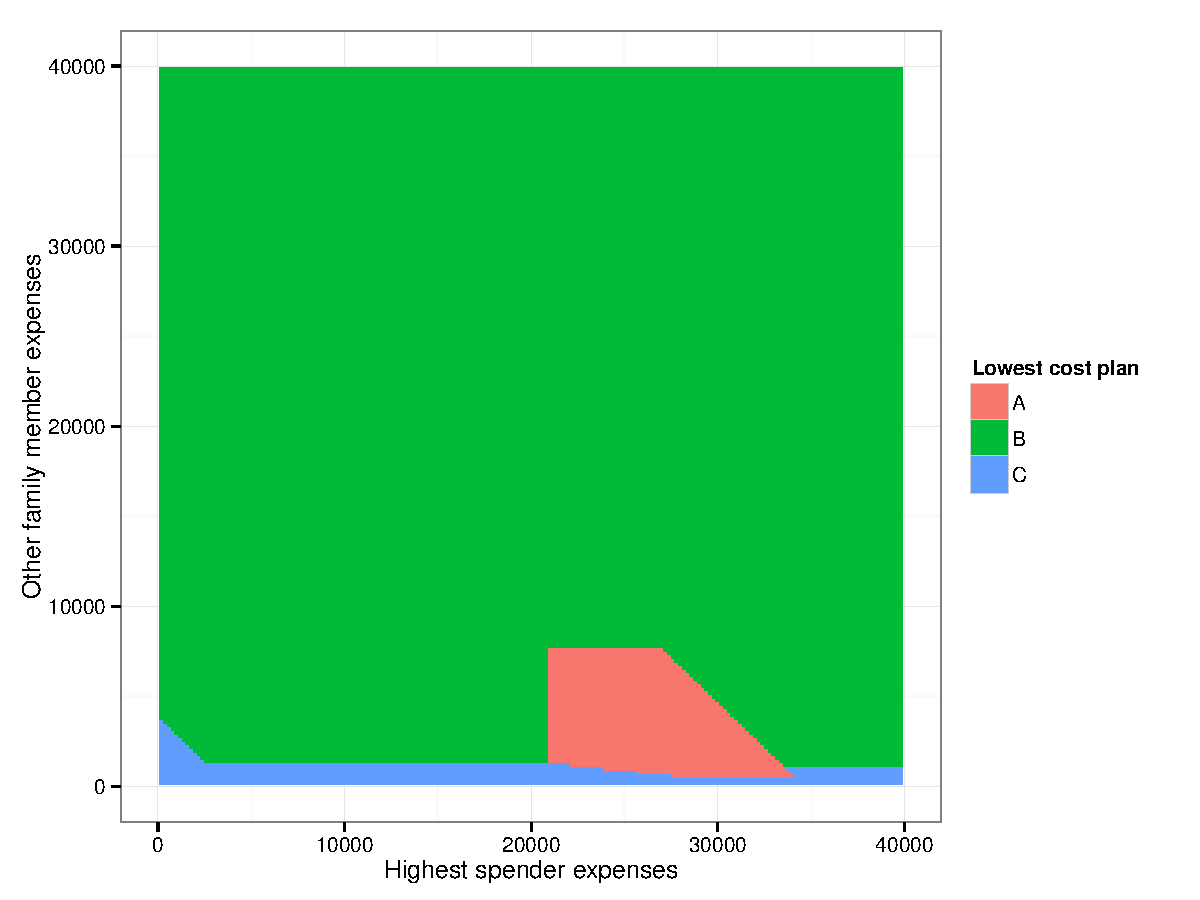
\includegraphics[height=6cm]{./img/ins-cost-map.pdf}
\end{center}
\end{frame}
\begin{frame}[fragile,label=sec-19]{Interaction was already on the horizon}
 \begin{itemize}
\item Demo showing \texttt{playwith} + \texttt{ggplot2}
\end{itemize}

\begin{center}
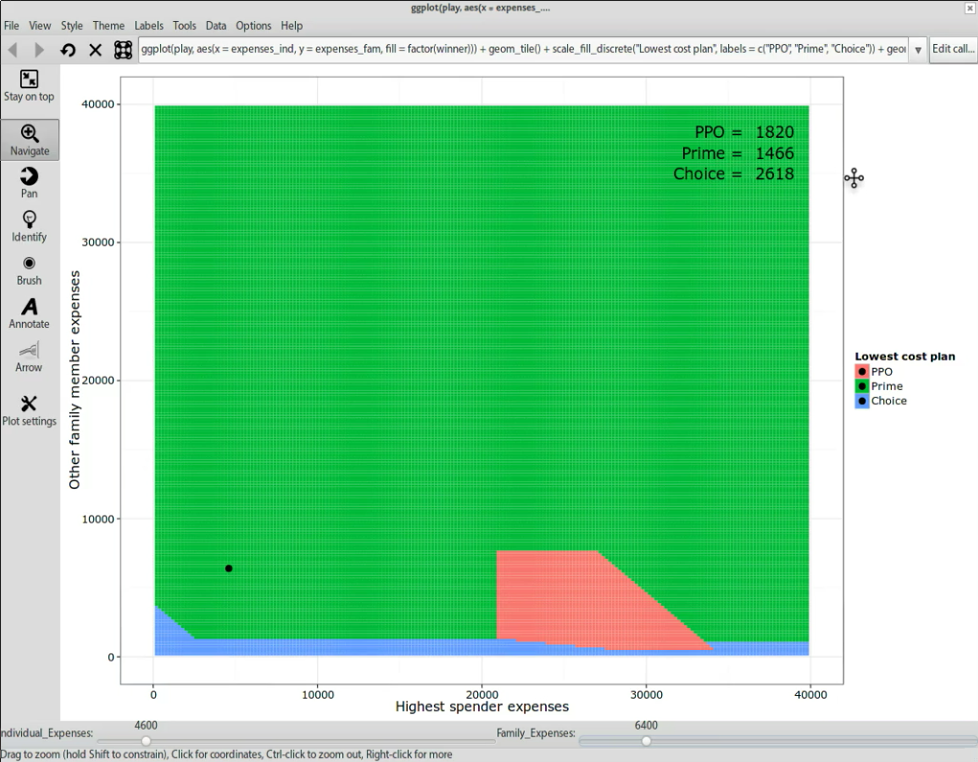
\includegraphics[height=6cm]{./img/ins-playwith.png}
\end{center}
\end{frame}
\begin{frame}[fragile,label=sec-20]{So, what about \emph{this} year?}
 \begin{itemize}
\item I used \texttt{shiny}, obviously!
\item Dynamic UI elements for \# of people on plan
\item \href{http://stackoverflow.com/questions/18116967/dealing-with-conditionals-in-a-better-manner-than-deeply-nested-ifelse-blocks}{"Interesting" algorithm} for dealing with complex criteria
\item A bit of \texttt{ggplot2} hackery
\item Hosted internally at 3M on \texttt{shiny} server
\item Put an anonymized version on \href{http://spark.rstudio.com/jwhendy/insurance-visualizer}{spark.rstudio.com}
\end{itemize}
\end{frame}
\begin{frame}[label=sec-21]{Table of possible outcomes}
\begin{center}
\tiny
\begin{center}
\begin{tabular}{rrrrrrrl}
\toprule
ded\(_{\text{ind}}\) & oop\(_{\text{ind}}\) & ded\(_{\text{rem}}\) & oop\(_{\text{rem}}\) & ded\(_{\text{tot}}\) & oop\(_{\text{tot}}\) & bin & formula\\
\midrule
0 & 0 & 0 & 0 & 0 & 0 & 0 & exp\(_{\text{ind}}\) + exp\(_{\text{rem}}\)\\
1 & 0 & 0 & 0 & 0 & 0 & 1 & ded\(_{\text{ind}}\) + 0.1 (exp\(_{\text{ind}}\) - ded\(_{\text{ind}}\)) + exp\(_{\text{rem}}\)\\
0 & 0 & 1 & 0 & 0 & 0 & 4 & exp\(_{\text{ind}}\) + exp\(_{\text{rem}}\)\\
1 & 0 & 0 & 0 & 1 & 0 & 17 & ded\(_{\text{ind}}\) + 0.1 (exp\(_{\text{ind}}\) - ded\(_{\text{ind}}\)) + exp\(_{\text{rem}}\)\\
1 & 1 & 0 & 0 & 1 & 0 & 19 & oop\(_{\text{ind}}\) + exp\(_{\text{rem}}\)\\
0 & 0 & 1 & 0 & 1 & 0 & 20 & ded\(_{\text{tot}}\) + 0.1 (exp\(_{\text{ind}}\) + exp\(_{\text{rem}}\) - ded\(_{\text{tot}}\))\\
1 & 0 & 1 & 0 & 1 & 0 & 21 & ded\(_{\text{tot}}\) + 0.1 (exp\(_{\text{ind}}\) + exp\(_{\text{rem}}\) - ded\(_{\text{tot}}\))\\
1 & 1 & 1 & 0 & 1 & 0 & 23 & oop\(_{\text{ind}}\) + ded\(_{\text{ind}}\) + 0.1 (exp\(_{\text{rem}}\) - ded\(_{\text{ind}}\))\\
1 & 0 & 1 & 1 & 1 & 0 & 29 & ded\(_{\text{tot}}\) + 0.1 (exp\(_{\text{ind}}\) + exp\(_{\text{rem}}\) - ded\(_{\text{tot}}\))\\
1 & 1 & 0 & 0 & 1 & 1 & 51 & oop\(_{\text{ind}}\) + exp\(_{\text{rem}}\)\\
1 & 1 & 1 & 0 & 1 & 1 & 55 & oop\(_{\text{ind}}\) + ded\(_{\text{ind}}\) + 0.1 (exp\(_{\text{rem}}\) - ded\(_{\text{ind}}\))\\
1 & 0 & 1 & 1 & 1 & 1 & 61 & oop\(_{\text{tot}}\)\\
1 & 1 & 1 & 1 & 1 & 1 & 63 & oop\(_{\text{tot}}\)\\
\bottomrule
\end{tabular}
\end{center}
\normalsize
\end{center}
\end{frame}
\begin{frame}[fragile,label=sec-22]{Break up expenses: highest vs. the rest}
 \scriptsize
\begin{verbatim}
converter <- function(expenses) {
  
  exp_ind <- max(expenses)
  exp_rem <- sum(expenses[-which(expenses == exp_ind)[1]])
  list("exp_ind" = exp_ind, "exp_rem" = exp_rem)
  
}
\end{verbatim}
\normalsize
\end{frame}
\begin{frame}[fragile,label=sec-23]{Check against criteria; convert to binary}
 \tiny
\begin{verbatim}
condition <- function(exp_ind, exp_rem, class) {
  
  compare <- plans[plans$class == class, ]
  
  test_case <- c(rep(c(exp_ind, exp_rem, exp_ind + exp_rem), each = 2))
  test_case <- rbind(test_case, test_case, test_case)
  
  limits <- cbind(compare$ded_ind, compare$exp_max_ind,
                  compare$ded_ind, compare$exp_max_ind, 
                  compare$ded_tot, compare$exp_max_tot)
  
  result <- cbind(compare[, c("ded_ind", "ded_tot", "oop_ind", "oop_tot", "prem", "hsa")],
                  exp_ind, exp_rem, (test_case > limits) %*% (2^(0:5)))
  names(result)[ncol(result)] <- "bin"
  return(result)
  
}
\end{verbatim}
\normalsize
\end{frame}
\begin{frame}[fragile,label=sec-24]{Hacky function lookup}
 \tiny
\begin{verbatim}
map_funcs <- list()
length(map_funcs) <- 17
map_funcs <- list(
  "0" = function(binary) { binary$exp_ind + binary$exp_rem }, 
  "1" = function(binary) { binary$ded_ind + (0.1* (binary$exp_ind - binary$ded_ind)) + binary$exp_rem }, 
  "4" = function(binary) { binary$exp_ind + binary$exp_rem }, 
  "16" = function(binary) { binary$ded_tot + (0.1 * (binary$exp_ind + binary$exp_rem - binary$ded_tot)) },
  "17" = function(binary) { binary$ded_ind + (0.1* (binary$exp_ind - binary$ded_ind)) + binary$exp_rem },
  "19" = function(binary) { binary$oop_ind + binary$exp_rem }, 
  "20" = function(binary) { binary$ded_tot + (0.1 * (binary$exp_ind + binary$exp_rem - binary$ded_tot)) }, 
  "21" = function(binary) { binary$ded_tot + (0.1 * (binary$exp_ind + binary$exp_rem - binary$ded_tot)) }, 
  "23" = function(binary) { binary$oop_ind + binary$ded_ind + (0.1 * (binary$exp_rem - binary$ded_ind)) },
  "28" = function(binary) { binary$ded_tot + (0.1 * (binary$exp_ind + binary$exp_rem - binary$ded_tot)) },
  "29" = function(binary) { binary$ded_tot + (0.1 * (binary$exp_ind + binary$exp_rem - binary$ded_tot)) },
  "48" = function(binary) { binary$oop_tot },   
  "51" = function(binary) { binary$oop_ind + binary$exp_rem }, 
  "55" = function(binary) { binary$oop_ind + binary$ded_ind + (0.1 * (binary$exp_rem - binary$ded_ind)) }, 
  "60" = function(binary) { binary$oop_tot }, 
  "61" = function(binary) { binary$oop_tot }, 
  "63" = function(binary) { binary$oop_tot }
)
\end{verbatim}
\normalsize
\end{frame}
\begin{frame}[fragile,label=sec-25]{Creating the right data to plot}
 \tiny
\begin{verbatim}
generate_plot_data <- function(binary) {
            
  plot <- lapply(1:nrow(binary), function(i) {
    temp <- binary[i, ]
    delta <- temp$cost - temp$hsa - hsa_vol
    plot <- data.frame(plan = rep(temp$plan, 4),
                       start = c(min(delta, 0),
                       temp$prem, max(0, delta),
                       c(temp$cost, temp$hsa)[(delta > 0)+1]))
    plot[plot$plan == "PPO", "start"][1] <- 0
    offsets <- c(0, cumsum(plot$start[2:4]))
    plot$end <- offsets - abs(plot$start)
    plot$start <- offsets
    plot$fill <- factor(c("c", "b", "a", "a"))
    plot$alpha <- factor(c(1, 1, 1, 0))
    return(plot)
  } )
            
}
\end{verbatim}
\end{frame}
\begin{frame}[fragile,label=sec-26]{The plot}
 \tiny
\begin{verbatim}
  p <- ggplot(plot, aes(x = plan, xend = plan,
                        y = start, yend = end,
                        colour = fill, alpha = alpha))
  p <- p + geom_segment(size = 35) + theme_bw()
  p <- p + coord_flip() + facet_wrap(~case, ncol = 2)
  p <- p + scale_alpha_discrete(range = c(0.35, 1), guide = F)
  p <- p + scale_colour_manual("Annual Cost", limits = c("a", "b", "c", "d"),
           labels = c("Expenses", "Premiums", "Carry-over HSA",
                      "Expenses paid \n from HSA/HCRA"),
           values = hcl(c(15, 255, 135, 15), l=65, c=100, alpha = c(1, 1, 1, 0.35)))
  p <- p + scale_y_continuous(limits = c(min(c(plot$start, plot$end)),
                                         max(c(plot$start, plot$end))),
           breaks = c(seq(-1000, max(plot$end, plot$start), by = 500)))
  p <- p + theme(axis.title = element_blank(), text = element_text(size = 20),
                 axis.text.x = element_text(angle = 315, hjust = 0))
  p <- p + guides(colour = guide_legend(override.aes = list(size = 7)))
  print(p)
\end{verbatim}
\normalsize
\end{frame}
\begin{frame}[label=sec-27]{}
\vfill
\begin{center}
'Nuff talk, let's take a look!
\end{center}
\vfill
\end{frame}
% Emacs 24.3.1 (Org mode 8.2.5h)
\end{document}
